\chapter{Implementation}\label{sec:impl}
Implementation of all three programs followed the same process, as outlined in Figure~\ref{fig:imp-flow}. The full process would take between three to four weeks to complete for each kernel. I first implemented BabelStream, then the sparse matrix vector multiplication kernel and finally the K-means kernel, in that order.

\begin{figure}[h]
  \center
  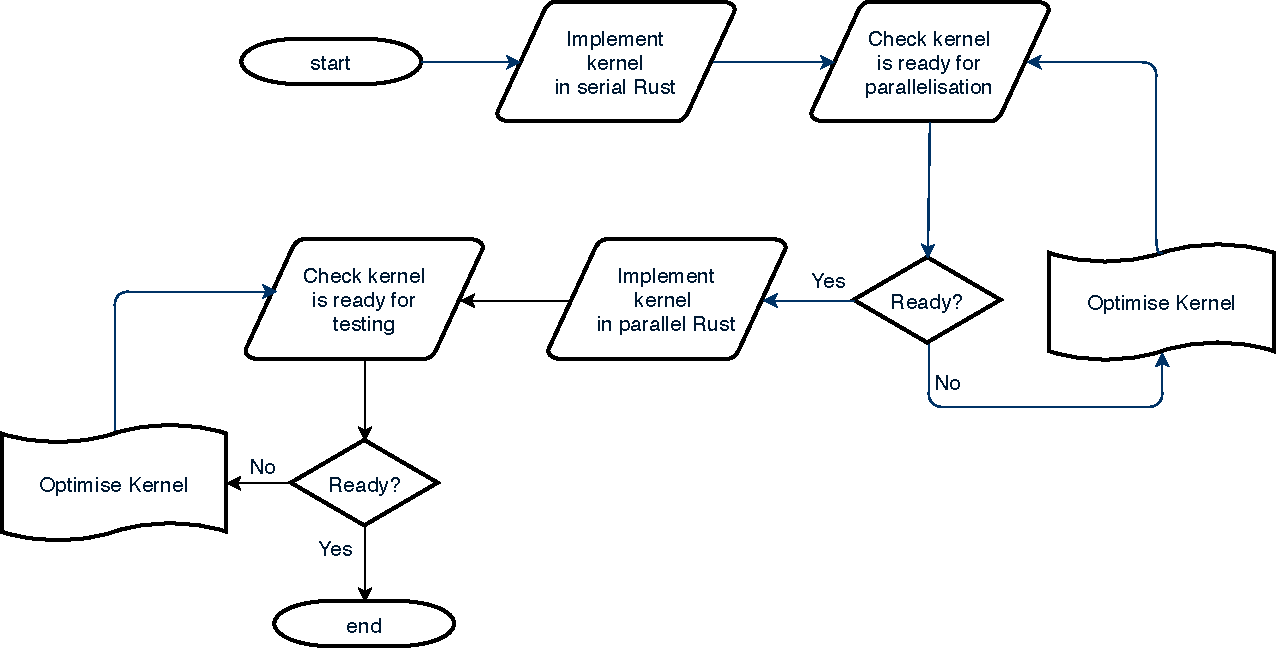
\includegraphics[width=\linewidth]{figs/ImplementationFlow.pdf}
  \caption{Flow diagram for implementation process}
  \label{fig:imp-flow}
\end{figure}

\section{Porting to Serial Rust}
Once a candidate kernel is selected, it is implemented in Rust in serial. Any differences between the  behaviour of the Rust and the original implementation are thought of as bugs, and are eradicated or minimised as far as is possible. For ease of development, the Rust crate Clap~\cite{RustClap} was used to read command line arguments for the program, leading to Rust implementations of kernels being called with different syntax. This difference was deemed to be superficial enough to be allowable. Kernel output was as similar as possible to aid data-collection from both implementations.

BabelStream was in some ways one of the hardest kernels to port to serial Rust. This was partly due to it being the first program which I attempted to port, but also because of Rust's type system and the use of generics. The original C++ implementation of the program uses templates to allow the user to choose to use 32 or 64 bit floating numbers when running the program. To achieve the same thing in Rust, generic types have to be used, which are defined through traits.

I found that using generics in Rust made reading error messages difficult, but easier to parse once the offending code was removed into a smaller example, and stripped of its generic type. Generics in Rust necessitate verbose syntax, for example, \texttt{T::from(0)} \texttt{.unwrap()} is used to generate a zero of type T. 
The first part of this expression generates an option type, which in this case is \texttt{Some(0.0)}, and is then unwrapped into simply \texttt{0.0}. Rust does this to allow programmers to deal with cases where a value of type T is impossible to generate from the input value, such as casting a value greater than $2^{32} - 1$ to a signed 32 bit value.
In this circumstance, the value returned would be \texttt{None}, which the programmer would then have to deal with. As zero can always be successfully cast to a 32 or 64 bit floating point number, it is safe to simply unwrap the value here, but if it was a number that could not be cast to the type, then the program would crash at this point. A C or C++ program doing the same thing, casting a 64 bit number to a 32 bit number would not crash, but its result would be implementation specific undefined behaviour, or throw an exception. This difference shows how Rust and C or C++ prioritise, and conceive of, safety.

The Rust implementation of Babel stream, like the reference implementation, creates a stream object which calls certain functions on its own data sets. This was quite easy to implement as Rust has enough features of object oriented programming, such as allowing objects to contain data and behaviour, for these simple objects to work.
However, Rust does not implement inheritance, which is considered by some to be a foundational aspect of object oriented programming~\cite{Liskov:1987}, which is also used by BabelStream. Rust instead uses trait objects to share behaviours. This design choice did not interfere with any of the simple kernels which were implemented, but would certainly be interesting to translate object inheritance from a larger program, maybe a mini-app, into Rust's trait feature.
Whilst the concept of borrowing did take some time to fully understand, I found that the compiler gave very helpful and accurate hints on how to make sure my program complied with the borrow checker. For example, in listing~\ref{lst:rustc-borrow}, the programmer is informed that they `cannot borrow `self.c' as mutable', and is shown where the function tries to mutate the value. 

\begin{code}
\begin{minted}{bash}
error[E0596]: cannot borrow 'self.c' as mutable, as it is behind a
              `&` reference
  --> src/stream.rs:20:9
   |
18 |     pub fn triad(&self){
   |                  ----- help: consider changing this to be a
    mutable reference: `&mut self`
20 |         self.c[0] = self.a[0] + self.b[0];
   |         ^^^^^^ 'self' is a '&' reference, so the data it refers
    to cannot be borrowed as mutable
error: aborting due to previous error
\end{minted}
\captionof{listing}{Rust Compiler: The borrow checker warns the programmer they can not access a variable as mutable}
\label{lst:rustc-borrow}
\end{code}

The stream object's triad function, which alters the objects data, but takes mutable ownership of the data, through using \texttt{\&mut self}, where \texttt{\&mut} is a mutable borrow. Once the programmer implements the compiler's suggested fix, this fragment of code will compile.

The sparse matrix vector multiplication kernel was quite simple to port to serial Rust, as I was able to ignore parts of the small program which would not be used, like the scramble function. As with BabelStream, I found converting from C's data types into Rust to be difficult due to Rust's safety constraints.
For example, in the C implementation, the vector holding the column index of the matrix was composed of values of type \texttt{s64Int}, which is a signed 64 bit integer. This datatype is directly analogous to Rust's \texttt{i64} data type, except in C you may use numbers of type \texttt{s64Int} to index into arrays, where as in Rust you must only use numbers of type \texttt{usize}. Errors of this type are easily dealt with however, as they are explicitly pointed out to the programmer at compile time, and can be remedied with casts in the simple format \texttt{as usize}. I found the SpMV kernel easier to port to serial Rust than BabelStream, but this could have been because I was already more familiar with Rust's way of doing things.

Although installing the dependencies for the reference implementation of the K-means clustering kernel was difficult, it was easy to get NetCDF working with Rust. I found a NetCDF Rust library~\cite{RustNetCDF}, which I added to my implementation's \texttt{Cargo.toml} file. I was then easily able to compile and use this library within my K-means implementation.

An interesting factor in writing the K-Means cluster in Rust was porting the original helper functions, which were used to make 2D integer and 2D float arrays. In the original C implementation, these 2D arrays were of type \texttt{float**} and \texttt{int**}.
When I was porting these data structures to Rust, it was important to consider if data locality impacted their use. The original implementation used the data in column wise operations, so that the next datum to be used was likely to have already been loaded in the same cache line as the previous one. This allowed me to write my implementation as a vector of \texttt{f32} or \texttt{i32} vectors.

The Rust vector of vectors was generated from a single one dimensional vector using the same algorithm as the reference implementation, where sections of the original vector are read into the new vectors within the vector of vectors. Although the original is well suited to C's memory management idioms, it was easy to write the same method in safe Rust. The ease with which I was able to re-implement this routine is another suggestion of Rust's ability to replace C's use in HPC.

\section{Serial Optimisation}
Next, I found and eliminated bugs in my serial implementation of the code by comparing outputs between my implementation and the reference implementation. During this process I would also move the code away from its C-style towards idiomatic Rust. To achieve more idiomatic Rust, I used the linting\footnote{A linter or linting tool checks that a programs syntax meets some standard} tool Clippy~\cite{RustClippy}, which was developed by the Rust team.  Clippy includes a category of lints  which highlight `code that should be written in a more idiomatic way'~\cite{RustClippy}. I implemented most of Clippy's recommended rewrites, which would often include replacing the use of for loops over integer indexes to access vector variables with calls to the vector's \texttt{iter()} method. This particular replacement requires code to be rewritten in a much more functional style.

For example, all of the array operations in BabelStream were originally written in a C-style, and then transformed to use iterators. Listing~\ref{lst:iters-b}, shows the original, more succinct for loop form of BabelStream's add operation. This style is rejected by Clippy, which prefers the style presented by listing~\ref{lst:iters-a}.

\noindent\begin{minipage}{.49\textwidth}
    \begin{code}
\begin{minted}{rust}
for i in 0..self.c.len() as usize {
    self.c[i] = self.b[i] + self.a[i]
}
\end{minted}
\captionof{listing}{Rust: BabelStream add, before applying idiomatic style}
    \label{lst:iters-b}
\end{code}
\end{minipage}\hfill
\begin{minipage}{.49\textwidth}
    \begin{code}
\begin{minted}[fontsize=\scriptsize]{rust}
for ((c, b), a) in self.c.iter_mut()
                 .zip(self.b.iter())
                 .zip(self.a.iter()){
    *c = *b + *a;
}
\end{minted}
\captionof{listing}{Rust: BabelStream add, after applying idiomatic style}
\label{lst:iters-a}
\end{code}
\end{minipage}

Whilst the more idiomatic rust style in listing~\ref{lst:iters-a} is less succinct than~\ref{lst:iters-b}, it does have some benefits which the C-style for loop does not possess. For example, if the stream object's c array had been of greater length than its \texttt{a} or \texttt{b} arrays, the more C-like implementation would fail at run time with an index out of bounds error, whereas the more idiomatic code only writes to as many elements of \texttt{c} as the least number of elements there are of any of the arrays it is zipped with.

Also note in listing~\ref{lst:iters-a} the distinction between the methods \texttt{iter()} and \texttt{iter\_mut()}, the first of which creates an iterator, and the second of which creates an iterator which may change (mutate) its elements. Although an in-depth investigation was not carried out to see if the compiler made use of any optimisations here from the greater amount of information available to it, the time to run this fragment did decrease when converted to idiomatic Rust, from 95 milliseconds to 90.

A bug in my sparse matrix vector multiplication implementation was found at this stage. When launched with certain parameters, the C version ran without error. The Rust version would {\em panic}\footnote{Rust uses the term panic for immediate program termination due to some error} and fail every time, whilst initilising the \texttt{col\_index} with the error message:


\begin{code}
\begin{minted}{bash}
thread 'main' panicked at 'attempt to shift left with overflow', main.rs:8:13
\end{minted}
\captionof{listing}{Rust Compiler: Bit shift overflow}
\label{lst:rutsc-bit}
\end{code}

The panic was occurring because although I had mirrored the types used by the reference implementation, the behaviour of those types differed. In the reference implementation, radius was of type \texttt{int}, which is a 32-bit integer. I therefore translated this into a \texttt{i32} type in Rust. These values are used as upper limits in an initialisation loop, where intermediate values of the same type are bit-shifted before being stored in the \texttt{col\_index} array. In C, the operation shown in the listing~\ref{lst:bit-shift} sets \texttt{foo} to 2, when all numbers are 32 bit integers. 
\begin{code}
\begin{minted}{c}
int foo = 1 << 33;
\end{minted}
\captionof{listing}{C: Bit shift overflow}
\label{lst:bit-shift}
\end{code}

This occurs because the value 1 overflows and rolls over, in most implementations. The standard does not define this behaviour. In Rust however, this code causes the program to panic and quit~\footnote{The compiler will catch this error before run time if it can calculate the value 1 will be shifted by}. The Rust language does not consider this behaviour to be strictly unsafe, but does think that that the programmer `should' find it `undesirable, unexpected or erroneous'~\cite{rustunsafe}.
However, Rust does recognise that some programs do rely upon overflow arithmetic, and provides mechanisms to enable this feature within safe Rust. I was not required to use this feature after changing radius from the \texttt{i32} type to \texttt{usize} type, which is 64 bits.
This choice was made because the radius values were being cast to \texttt{usize} more often than they were being used as \texttt{i32}. This had the consequence of making the program impossible to bit shift overflow, as a radius of 64 requires a stencil diameter greater than $2^{32}-1$, which would in turn require a \texttt{col\_index} array terabytes in size, which the Cirrus hardware does not support.

When this optimisation pass was applied to K-means, it showed the limits of Clippy's linter. Clippy flagged concise for loops with warnings, and suggested verbose rewrites of them. For example, on line 110 of the kernel, just before the second part of the maximisation is about to begin, Clippy complains that listing~\ref{lst:for-concise} has a `needless range loop'.

\begin{code}
\begin{minted}{rust}
for k in 1..clusters_d.len as usize {
\end{minted}
\captionof{listing}{Rust: Needless range loop identified by Clippy}
\label{lst:for-concise}
\end{code}
Clippy argues this pattern should be avoided, because `iterating the collection itself makes the intent more clear and is probably faster'~\cite{ClippyLoop}. However, its suggested replacement is much longer, and the deeply chained methods take longer to comprehend.
\begin{code}
\begin{minted}{rust}
for (k, <item>) in old_cluster_centres.iter()
                                       .enumerate()
                                       .take(clusters_d.len as usize)
                                       .skip(1) {
\end{minted}
\captionof{listing}{Rust: Clippy's suggested verbose iterator is hard to read}
\end{code}
It would be difficult to argue that the code suggested by Clippy is idiomatic, as idiomatic code is generally agreed to be code which uses features of the language to achieve conciseness. This code fragment is clearly not concise, and I therefore did not make Clippy's suggested correction.
\section{Parallelisation}
I then parallelised the kernel with Rayon (Section~\ref{sec:back-rayon}), at the same loops where the reference implementation uses OpenMP\@. Sometimes this would little more than replacing the \texttt{iter()} method with \texttt{par\_iter()}, but parallelising more complex operations like reductions and initialisation was more difficult.

Parallelising BabelStream was simple. As listing~\ref{lst:iters-p} shows, BabelStream's add operation remains largely the same, only that the \texttt{iter()} method has been replaced by the \texttt{par\_iter()} method, and that the method \texttt{for\_each} has to be called. As the serial version of this loop had no inter loop dependencies, it could easily be transformed from a for loop to a parallel for each loop.
\begin{code}
\begin{minted}{rust}
self.c.par_iter_mut()
            .zip(self.b.par_iter())
            .zip(self.a.par_iter())
            .for_each(|((c, b), a)| *c = *a + *b);
\end{minted}
\captionof{listing}{Rust: BabelStream add, parallelised using Rayon's for each method.}
\label{lst:iters-p}
\end{code}

This pattern was applicable to the copy, multiply, add, and triad methods. The dot method needed more alteration than these methods to be parallelised, as the original, Clippy compliant code was very different to the final code used. The original code in Listing~\ref{lst:dot-for} updates the sum value from within a for loop before returning it.
\begin{code}
\begin{minted}[fontsize=\scriptsize]{rust}
let mut sum1: T = T::from(0).unwrap();
for (a, b) in self.a.iter()
                    .zip(self.b.iter()){
                      sum1 += a * b;
                    }
sum1
\end{minted}
\captionof{listing}[Rust: Serial dot product]{Rust: Serial dot product. The value \texttt{sum1} is the accumulator.}
\label{lst:dot-for}
\end{code}
This update pattern does not work with a Rayon parallel for each loop, as threads are not able to write to a shared variable. The Rust compiler gives the error that the closure does not implement \texttt{FnMut}, which is `The version of the call operator that takes a mutable receiver'~\cite{rust-doc-fnmut}. A mutable receiver in this case refers to a mutable variable which is created, and lives on, outside of the iterator's scope. This error demonstrates the utility of Rust's mutable and immutable variables in parallel operations, allowing the programmer to avoid the read modify write dataa race seen earlier in the OpenMP example in listing~\ref{lst:omp-eg}.

To solve this error, the expression is rewritten using the fold method. It was quite difficult to find exactly how to write this, as the serial fold method has a different call signature to the Rayon parallel fold. The final implementation of BabelStream's fold is shown in listing~\ref{lst:dot-fold}.
\begin{code}
\begin{minted}[fontsize=\scriptsize]{rust}
let sum1: T = T::from(0).unwrap();
self.a.par_iter()
    .zip(self.b.par_iter())
    .fold(|| sum1, |acc, it| acc + *it.0 * *it.1).sum()
\end{minted}
\captionof{listing}[Rust: Parallel dot product]{Rust: Parallel dot product, using \texttt{fold()} to create a partial sum which is reduced.}
\label{lst:dot-fold}
\end{code}
In this listing, a zero of type T is generated, and the vectors a and b are zipped together, as before. The fold method then takes two arguments, both of which are closures, or anonymous functions. The first closure is used to create the initial value, which is the value which can be used as the initial accumulator value when the zipped vector of \texttt{a} and \texttt{b} is divided between threads. The zipped vector of \texttt{a} and \texttt{b} takes the form

\begin{center}
$[(a_1, b_1), (a_2, b_2), \ldots, (a_{n-1}, b_{n-1})]$
\end{center}

The fold is applied to thread local subsections of this, resulting in the form:

\begin{center}
$[ [a_{t_{1}1} b_{t_{1}1} + a_{t_{1}2}b_{t_{1}2} + \ldots ], \ldots ,[\ldots + a_{t_{n-1}{n-2}} b_{t_{n-1}{n-2}} + a_{t_{n-1}{n-1}} b_{t_{n-1}{n-1}}] ]$ 
\end{center}
Where $t_n$ is a thread number. This is finally reduced to the a single number, through calling \texttt{sum()}

\begin{center}
$a_{t_{1}1} b_{t_{1}1} + a_{t_{1}2}b_{t_{1}2} + \ldots + a_{t_{n-1}{n-2}} b_{t_{n-1}{n-2}} + a_{t_{n-1}{n-1}} b_{t_{n-1}{n-1}}$ 
\end{center}

Although the initial change of perspective required to use Rayon's fold was confusing, especially because it can sometimes function more like a map, once the cognitive leap had been made the simplicity was clear. Although it was hard to use Rayon's fold method, I did not find it to be prohibitively difficult.

Most of the methods of BabelStream were easy to parallelise, but this does not necessarily show us the expressiveness of the Rayon library. The parallelised methods were so simple that they were extremely unrepresentative of production HPC code. The sparse matrix vector multiplication parallelisation was more representative of the type of parallelism which is done in HPC, and was therefore more complex than BabelStream. Even so, parallelising the central processing loop of SpMV was trivial.
\noindent\begin{minipage}{.49\textwidth}
\begin{code}
\begin{minted}[fontsize=\scriptsize]{rust}
for row in 0..size2 as usize {
  let first = stencil_size * row;
  ...
  result[row] += temp;
}
\end{minted}
\captionof{listing}[Rust: Serial SpMV.]{Rust: Serial SpMV. \texttt{first} sets the bound for that row's reduction to the result.}
\end{code}
\end{minipage}\hfill
\begin{minipage}{.49\textwidth}
\begin{code}
\begin{minted}[fontsize=\scriptsize]{rust}
result.par_iter_mut()
      .enumerate()
      .for_each( |(row, item)| {
  let first = stencil_size * row;
  ...
  *item += temp;
}
\end{minted}
\label{lst:spmv-par}
\captionof{listing}[Rust: Parallel SpMV\@.]{Rust: Parallel SpMV\@. To generate a value for \texttt{row} as in the serial implementation, \texttt{enumerate()} is used}
\end{code}
\end{minipage}

In the parallel version of the spare matrix vector multiplication I created a parallel mutable iterator over the result vector, and enumerated it. This allowed me to access the items and the indexes of the vector, which I used without changing the internal logic of the for loop at all. The applicability of this common HPC pattern from C into Rust indicates that Rust is an expressive language for HPC.

The K-means kernel's Expectation stage, or E-step, was harder to parallelise. This difficulty arose from trying to do two, seemingly mutually exclusive things, within the same loop. The code required me to update the values of the array and perform a reduction on another variable external to the loop. I had encountered the difficulty of reducing to a shared variable from multiple threads before, with BabelStream's dot product (see Listing~\ref{lst:dot-fold}), but was unaware of how to perform this reduction with side effects.

After some experimentation, I found the solution, a simple \texttt{map()} and then \texttt{sum()}. 

\begin{minipage}{.49\textwidth}
\begin{code}
\begin{minted}[fontsize=\scriptsize, frame=single]{rust}
for (idx, item) in x.iter()
                    .enumerate(){
    ...
    labels[idx] = k_best;
    dist_sum_new += dist_min;
}
\end{minted}
\captionof{listing}[Rust: K-means serial E-step]{Rust: K-means serial E-step. Each time a label's value is set, \texttt{dist\_sum\_new} is updated}
\label{lst:kmeansserial}
\end{code}
\end{minipage}\hfill
\begin{minipage}{.49\textwidth}
\begin{code}
\begin{minted}[fontsize=\scriptsize, frame=single]{rust}
dist_sum_new = labels.par_iter_mut()
                .enumerate()
                .map(|(idx, item)| {
    item = k_best;
    dist_min
    }).sum();
\end{minted}
\captionof{listing}[Rust: K-means parallel E-step]{Rust: K-means parallel E-step. Here, \texttt{dist\_sum\_new} is only updated once all the labels have been written to.}
\label{lst:kmeanspar}
\end{code}
\end{minipage}

In Listing~\ref{lst:kmeansserial} I am creating an iterator over \texttt{x}, which is a vector of the length as the vector \texttt{labels}. I had originally chosen this vector to be the one which created the iterator merely for convenience. I had to change this vector to \texttt{labels} in the parallel implementation however, as it is the items of \texttt{labels} that need to be updated. I then used the index value to retrieve the necessary values from \texttt{x} to calculate the value of \texttt{k\_best}. The value of \texttt{dist\_min} is also calculated for that particular index value. These \texttt{dist\_min} values are left in a map structure, which is reduced by the sum and written to \texttt{dist\_sum\_new}, yielding the same result as the serial implementation. 

This map and reduce operation seems to be particularly flexible, and after using the similar fold and then sum combination, was easier to conceive of. Whilst I did experience some difficulties in parallelising these programs with Rayon, it did feel like part of the difficulty was not the language's fault, but rather my lack of understanding of it.


\section{Parallel Optimisation}
Once I had parallelised the Rust implementations, I carried out another optimisation pass. This optimisation pass allowed me to find issues caused by parallelism, and make improvements only possible through parallelism. One such improvement was parallel initialisation.

Parallel initialisation is an important feature of programs which run on cache coherent non uniform memory access (CC-NUMA) systems. CC-NUMA systems often use a first touch allocation policy, which means that the page which is written to, is located near to the processor which first touched it. The 18 core Intel Xeon processors on Cirrus use this particular memory allocation policy, which therefore means that `poorly written applications (e.g., initializations  performed  at  a  single  processor  before  main  parallel computation  begins)  will  locate  pages  incorrectly based  on  the  first  access  and  cause  several  remote memory accesses later'~\cite{Bhuyan:2000}. Without parallel initialisation, the Rust implementation of BabelStream falls under this definition of a poorly written application. Preliminary testing had also found that the Rust implementation's performance had failed to scale past 8 threads, whilst the C++ implementation's performance continued to increase up to 24 threads. 

I had not yet written parallel initialisation in Rust as there was no clear way to do it. This was largely because in the C++ form of parallel initialisation, allocating the memory to be used and then initialising that memory are two distinct steps, where as in Rust they are the same step.

\noindent\begin{minipage}{.49\textwidth}
\begin{code}
\begin{minted}{c}
#pragma omp parallel for
for (int i = 0; i < array_size; i++)
{
    a[i] = initA;
    b[i] = initB;
    c[i] = initC;
}
\end{minted}
\captionof{listing}{C: BabelStream parallel initialisation}
\label{lst:serialInit}
\end{code}
\end{minipage}\hfill
\begin{minipage}{.49\textwidth}
\begin{code}
\begin{minted}{rust}
vec![0.0; arr_size].par_iter()
       .map(|_| T::from(0.2).unwrap())
       .collect_into_vec(&mut self.b);
\end{minted}
\captionof{listing}{Rust: BabelStream parallel initialisation}
\label{lst:parInit}
\end{code}
\end{minipage}

Listing~\ref{lst:serialInit} shows how the C++ version of BabelStream carries out its first touch in parallel, by adding a simple \texttt{\#pragma} statement to the code. This pattern is not reproducible with Rayon, as it doesn't use parallel for loops, but instead uses parallel iterators. The solution was found to be using the map function to collect values into a vector, as shown in listing~\ref{lst:parInit}.

This routine works by using the \texttt{vec!} macro to create a vector of length \texttt{arr\_size}, where every value in the vector is 0.0. This vector is then used to generate a parallel iterator. The parallel iterator performs a map, taking all values from the vector, and generating a corresponding value of 0.2, of type T. The \texttt{|\_|} notation here means that although the closure signature requires a value, that value will not be used in the closure's method.
These values of 0.2 are then collected into the vector held in \texttt{self.b}.

The use of map here to generate values for parallel initialisation seems like it is an unlikely use case scenario, but I discovered how to use it from the Rayon documentation on the map method~\cite{rayonIter}. Whilst clear documentation always helps a language to become more accepted, this use case was shown to not be as flexible as was needed by all kernels which were ported to Rust, as was found later when attempting to implement parallel initialisation for SpMV.

Figure~\ref{fig:babel-dot-init} shows the use of parallel initialisation greatly improved the memory bandwidth of the BabelStream. However, the improvement in performance still did not bring it to a parity with the C++ and OMP implementation, for reasons discussed further in section~\ref{sec:res-babel}.

\begin{figure}[H]
    \centering
    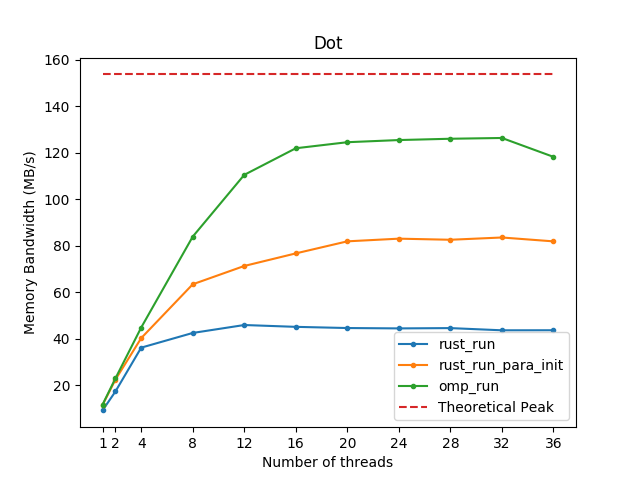
\includegraphics[width=.8\linewidth]{figs/babel/dot-init.png}
    \caption{BabelStream --- Dot product bandwidth initialisation comparison}
    \label{fig:babel-dot-init}
\end{figure}


The initialisation routine for the SpMV kernel was not as easy to implement. The difficulty was that the parallel loop used to write to elements of the vector \texttt{col\_index}, wrote to the vector in chunks of five. This made it very hard to translate into Rust, as Rayon only uses parallel iterators, and has no exact equivalent of parallel for loops.

Within an iterator, the programmer may only access the current element of the array, and the next element of the array. This restricted functionality is not expressive enough for the initialisation routine shown in listing~\ref{lst:sparseParaInit}, as I am unable to step in fours, and I am unable to access the next element of the vector without starting the iterator routine from its first instruction again.


\begin{code}
\begin{minted}{c}
#pragma omp for private (i,j,r)
for (row=0; row<size2; row++) {
j = row/size; i=row%size;
elm = row*stencil_size;
colIndex[elm] = REVERSE(LIN(i,j),lsize2);
    for (r=1; r<=radius; r++, elm+=4) {
      colIndex[elm+1] = REVERSE(LIN((i+r)%size,j),lsize2);
      colIndex[elm+2] = REVERSE(LIN((i-r+size)%size,j),lsize2);
      colIndex[elm+3] = REVERSE(LIN(i,(j+r)%size),lsize2);
      colIndex[elm+4] = REVERSE(LIN(i,(j-r+size)%size),lsize2);
    }
...
}
\end{minted}
\captionof{listing}{SpMV C Parallel Initilisation}
\label{lst:sparseParaInit}
\end{code}

Several methods were used in an attempt to solve this problem, including creating an object external to the iterable collection, which would be able to be updated between iterations. However, this method was unsuccessful as the Rayon iterator's did not implement \texttt{FnMut}. This problem was ultimately solved using Rust's parallel primitives:

\begin{itemize}
    \item \texttt{Mutex} - Protects shared data through mutual exclusion of locks.
    \item \texttt{channel} - Used to send data between threads.
    \item \texttt{Arc} - An atomic reference counter, which provides shared ownership of a value between threads.
    \item \texttt{thread} - The most basic threading model available in Rust. Platform agnostic.
\end{itemize}

These primitives were then used to initialise the \texttt{col\_index} array as follows.

\begin{enumerate}
    \item The main thread creates a vector, and wraps it in a \texttt{Mutex} which is wrapped in an \texttt{Arc}, which is labelled \texttt{col\_index}
    \item The main thread uses the \texttt{channel} to create a sender and a receiver nodes.
    \item The main thread enters a loop, where it creates \texttt{n} clones worth of \texttt{col\_index} constructs and sender nodes, where \texttt{n} is the total number of threads. The main thread then moves these constructs and nodes into the spawned threads. Each thread is given a consecutive thread ID starting from 0.
    \item Each thread calculates the section of \texttt{col\_index} it will write to from its thread ID and the size of the overall \texttt{col\_index}. This section is called \texttt{my\_col\_index}, and is created as a vector of zeros of the correct length for that thread and filled with zeros, which are then overwritten according to the original algorithm.
    \item Each thread then attempts to aquire the lock for the shared \texttt{col\_index}, and checks the length of it.
    \begin{enumerate}
        \item If the length of \texttt{col\_index} is the same as the lower bound of that thread's section, then the thread appends its \texttt{my\_col\_index} to \texttt{col\_index}, which it then releases the lock for.
        \item Otherwise, the releases the lock and periodically re-acquires it until \texttt{col\_index} is the right length.
    \end{enumerate}
\item Once the last thread has appended their \texttt{my\_col\_index} to \texttt{col\_index}, it sends an empty message to the master thread.
\item The master thread, which has been blocking, receives this message, and joins all the child threads. It then acquires the lock for \texttt{col\_index} and unwraps it, so that it can now be used as a normal vector.
\end{enumerate}

This whole routine is 62 lines of code, which is more than four times the original 16 lines of code. It was hard to find this solution, as requiring threads to operate in a specific order is not a typical use case scenario. 
The solution is complex, and brittle. Its verbosity makes it harder to read than the original code, and the need for careful array calculations feels unfaithful to the Rust philosophy of safety.

When implementing this solution, I kept running into array index out of bounds errors, implying that I was trying to write outside the array boundaries. These errors would crash the program. The cause of this issue was traced to the original implementation of the program, in C. I found this error by checking the final index written to by the threads, which was two more than the length of the array, if the program was run with certain input parameters. This error goes unnoticed in the C version of SpMV, because whilst a write overrun of 16 bits can cause a program to crash, on a modern system like Cirrus it is unlikely to. However, this is undefined behaviour and cannot be relied upon. I corrected my program's threads to write only within the boundaries of their vectors, and filed an issue for this bug on the ParRes Kernels' GitHub repository~\footnote{https://github.com/ParRes/Kernels/issues/405}.

Despite the negatives of the Rust version of the parallel initialisation, I did not find any bugs in it. Figure~\ref{fig:sparse-speedup} shows the benefit of implementing parallel initialisation for SpMV, which gives the Rust version better scaling than the C version, although its final speed is still slower than the C version's final speed. This difference will be discussed in more detail in section~\ref{sec:res-sparse}

\begin{figure}[H]
    \centering
    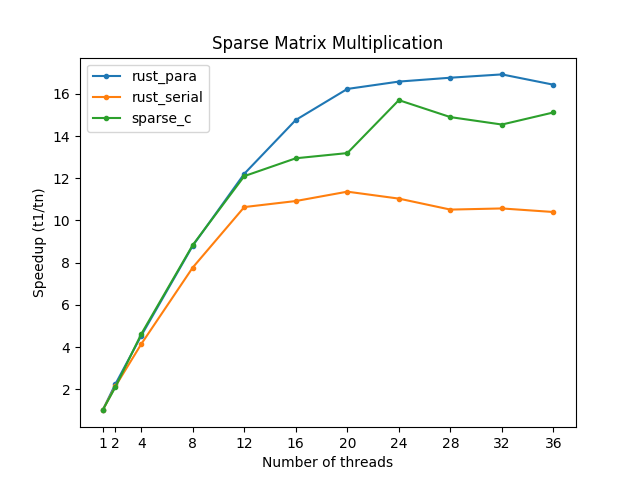
\includegraphics[width=.8\linewidth]{figs/sparse/speedup.png}
    \caption[SpMV --- Speed up]{SpMV speed up comparison against number of threads shows parallel initilisation scales better than serial.}
    \label{fig:sparse-speedup}
\end{figure}

The K-means kernel did not use any parallel initialisation, and therefore did not undergo parallel optimisation.
